{
% Set the overall layout of the tree
\tikzstyle{level 1}=[level distance=2.5cm, sibling distance=2cm]
\tikzstyle{level 2}=[level distance=2.5cm, sibling distance=2cm]

% Define styles for bags and leafs
\tikzstyle{bag}=[rectangle,draw=black,text width=4em,text centered]
\tikzstyle{end}=[circle,draw=black,minimum width=3pt,fill,inner sep=0pt]

\begin{figure}
	\centering
	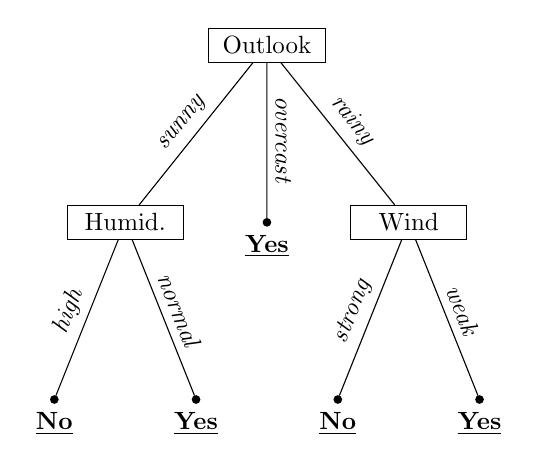
\begin{tikzpicture}[
		scale=0.9,
		every node/.style={scale=0.9},
		sloped
	]
		\node[bag]{\highlighttt{Outlook}}
    		child {
        			node[bag]{\highlighttt{Humid.}}        
        			child {
            		    	node[end,label=below:{\textbf{\underline{No}}}]{}
            		    	edge from parent
            		  	node[above]{\textit{high}}
            		}
            		child {
                			node[end,label=below:{\textbf{\underline{Yes}}}]{}
                			edge from parent
                			node[above]{\textit{normal}}
            		}
        			edge from parent         
            		node[above]{\textit{sunny}}
		}
		child {
			node[end,label=below:{\textbf{\underline{Yes}}}]{}
			edge from parent
			node[above]{\textit{overcast}}
		}
		child {
        			node[bag]{\highlighttt{Wind}}        
            		child {
                			node[end,label=below:{\textbf{\underline{No}}}]{}
                			edge from parent
                			node[above]{\textit{strong}}
            		}
            		child {
                			node[end,label=below:{\textbf{\underline{Yes}}}]{}
               			edge from parent
                			node[above]{\textit{weak}}
            		}
            		edge from parent 
            		node[above]{\textit{rainy}}
    		};
	\end{tikzpicture}
\end{figure}}